\section{Method}\label{sec:method}

Fig.~\ref{fig:overview} gives an overview. The three layers differ only in how features are constructed; the learning and evaluation protocol is shared, which is what makes the layers comparable.

\begin{figure*}[t]
\centering
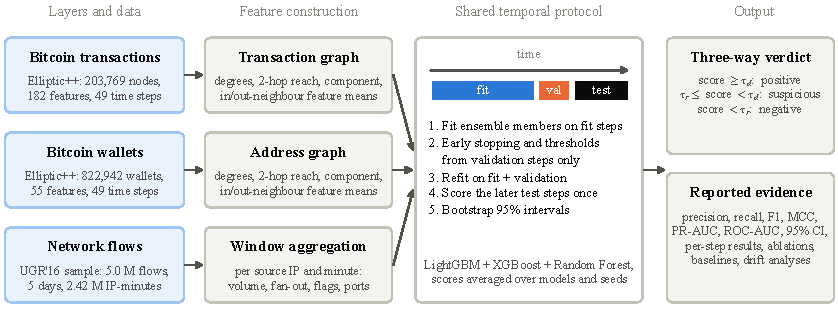
\includegraphics[width=\textwidth]{figures/fig_overview.pdf}
\caption{The three detection layers and the shared protocol. Feature construction is layer-specific; model fitting, threshold selection, the three-way verdict and all reported evidence follow one procedure in which the test period is used exactly once.}\label{fig:overview}
\end{figure*}

\subsection{Graph-derived features for transactions and wallets}\label{sec:method-graph}
Let $G = (V, E)$ be the directed transaction graph or address graph, $A$ its adjacency matrix with $A_{ij} = 1$ if $(i, j) \in E$, and $\mathcal{N}^{\mathrm{in}}(i)$, $\mathcal{N}^{\mathrm{out}}(i)$ the in- and out-neighbours of node $i$. Missing feature values are replaced by medians computed on the training period. Each node is then described by
\begin{equation}\label{eq:features}
\mathbf{z}_i = \big[\, \mathbf{x}_i ,\; \mathbf{g}_i ,\; \mathbf{m}^{\mathrm{in}}_i ,\; \mathbf{m}^{\mathrm{out}}_i \,\big],
\end{equation}
where the neighbourhood means are
\begin{equation}\label{eq:mean}
\mathbf{m}^{\mathrm{in}}_i = \frac{1}{|\mathcal{N}^{\mathrm{in}}(i)|} \sum_{j \in \mathcal{N}^{\mathrm{in}}(i)} \mathbf{x}_j ,
\end{equation}
and $\mathbf{m}^{\mathrm{out}}_i$ is defined analogously over $\mathcal{N}^{\mathrm{out}}(i)$. A node without neighbours in a direction receives a missing value for that block, which the tree learners treat as a category of its own. The vector $\mathbf{g}_i$ holds nine structural descriptors: in-degree $d^{\mathrm{in}}_i$, out-degree $d^{\mathrm{out}}_i$, their sum $d_i$, the ratio $d^{\mathrm{out}}_i / (d_i + 1)$, the two-hop walk counts $(A^{\top} \mathbf{d}^{\mathrm{in}})_i$ and $(A\, \mathbf{d}^{\mathrm{out}})_i$, the mean total degree of in- and of out-neighbours, and $\log(1 + c_i)$ with $c_i$ the size of the weakly connected component of $i$. This yields $3d + 9$ features: 555 for transactions ($d = 182$) and 174 for wallets ($d = 55$).

Equation~\eqref{eq:mean} is the mean aggregator of GraphSAGE~\cite{hamilton2017} applied once, without learned weights and computed before training. Only features are propagated. Labels of neighbours are never used as inputs, because at decision time the labels of contemporaneous entities are unknown.

\subsubsection{Transductive and causal neighbourhoods} Equation~\eqref{eq:mean} averages over all neighbours of $i$, including nodes with a later time index. For transactions this is immaterial, since edges connect transactions of the same time step (Section~\ref{sec:res-graph}). For wallets it means that a training wallet's features can depend on wallets that first appear in the test period. To measure whether results depend on this, we also evaluate a \emph{causal} variant in which the sums run only over neighbours that already exist,
\begin{equation}\label{eq:causal}
\mathcal{N}^{\mathrm{in}}_{\mathrm{c}}(i) = \{\, j \in \mathcal{N}^{\mathrm{in}}(i) : t_j \le t_i \,\},
\end{equation}
and likewise for out-neighbours.

\subsection{Behaviour windows for network flows}\label{sec:method-net}
A single flow record carries little evidence, and attack behaviour such as scanning is a property of many flows from one origin. Flows are therefore grouped by source address $a$ and by consecutive windows of $w = 60$ seconds, and each non-empty group $F_{a,k}$ becomes one entity. Its 32 features describe volume (flows, packets, bytes, their ratios, mean and maximum duration), fan-out (numbers of distinct destination addresses, destination ports and source ports, and their ratios to the flow count), protocol shares (TCP, UDP, ICMP), TCP-flag shares (SYN, SYN without ACK, RST, FIN), port usage (shares of flows to ports 22, 23, 25, 53, 80, 443 and to ports below 1024), the share of single-packet flows, and the hour of day. A window is positive if it contains at least one flow labelled as an attack. Windows whose only non-background flows are labelled \texttt{blacklist} are excluded from training and evaluation, because that label marks membership of an address in a blacklist and not observed behaviour; they are still scored.

The stream is read in chunks, so the raw file is never held in memory. All positive windows are kept; background windows may be retained with probability $r$ to bound memory. With $r < 1$, recall and the false-positive rate are unaffected in expectation, but precision is inflated. We then also report
\begin{equation}\label{eq:padj}
\tilde{P} = \frac{\mathrm{TP}}{\mathrm{TP} + \mathrm{FP}/r} ,
\end{equation}
which rescales false positives to the full background. The main network experiment uses $r = 1$; a run with $r = 0.25$ is reported in Section~\ref{sec:res-net} to show how the sampling rate affects the operating point.

\subsection{Ensemble}\label{sec:method-ens}
The detector averages the scores of three tree learners, each trained with several random seeds:
\begin{equation}\label{eq:ens}
\hat{s}(\mathbf{z}) = \frac{1}{|\mathcal{M}|} \sum_{m \in \mathcal{M}} \frac{1}{|\mathcal{S}_m|} \sum_{k \in \mathcal{S}_m} f_{m,k}(\mathbf{z}),
\end{equation}
with $\mathcal{M}$ = \{LightGBM~\cite{ke2017}, XGBoost~\cite{chen2016}, Random Forest~\cite{breiman2001}\} and $f_{m,k}$ the estimated probability of the positive class from learner $m$ with seed $k$. Averaging was chosen over stacking because a meta-learner would need a further held-out period, and the available validation periods are short.

\subsection{Temporal protocol}\label{sec:method-protocol}
Let $T_f < T$ split the training period into a \emph{fit} part ($t \le T_f$) and a \emph{validation} part ($T_f < t \le T$). The protocol has four stages.

\subsubsection{Fit} Every learner is trained on the fit part. The boosted learners use early stopping on validation PR-AUC, which yields a number of rounds $R_{m,k}$.

\subsubsection{Select thresholds} With $\hat{s}$ computed on the validation part $\mathcal{D}_{\mathrm{val}}$, the \emph{decision threshold} maximises the F1 score of the positive class,
\begin{equation}\label{eq:taud}
\tau_d = \underset{\tau}{\arg\max}\; F_1\big(\tau ;\, \mathcal{D}_{\mathrm{val}}\big),
\end{equation}
and the \emph{review threshold} is the largest threshold that still retrieves a fraction $\rho$ of the validation positives, capped by $\tau_d$:
\begin{equation}\label{eq:taur}
\tau_r = \min\Big( \tau_d ,\; \max\{\tau : \mathrm{Recall}(\tau ;\, \mathcal{D}_{\mathrm{val}}) \ge \rho \} \Big), \quad \rho = 0.95 .
\end{equation}

\subsubsection{Refit} Each learner is retrained on fit and validation together, so that the most recent labelled period is not wasted. Boosted learners run for $\lceil \gamma R_{m,k} \rceil$ rounds with $\gamma = \min(n_{\mathrm{train}} / n_{\mathrm{fit}},\, 1.25)$, a mild increase that reflects the larger training set. Thresholds are not re-estimated.

\subsubsection{Test} The refitted ensemble scores all entities once. An entity receives the verdict
\begin{equation}\label{eq:verdict}
v_i = \begin{cases} \text{positive} & \hat{s}_i \ge \tau_d \\ \text{suspicious} & \tau_r \le \hat{s}_i < \tau_d \\ \text{negative} & \hat{s}_i < \tau_r . \end{cases}
\end{equation}
The \emph{positive} verdict is the binary decision on which precision, recall and F1 are computed. The \emph{suspicious} band is intended as a queue for manual review. Nothing computed on $t > T$ influences a model, a threshold or a reported configuration.

\subsection{Reference models}\label{sec:method-baselines}
Three references are trained under the same protocol on the original features $\mathbf{x}_i$ only: (i) logistic regression on quantile-normalised features with balanced class weights; (ii) Isolation Forest~\cite{liu2008}, fitted on the negative class of the training period and therefore unsupervised with respect to the positive class; and (iii) a Random Forest with 50 trees and default settings, the strongest model of~\cite{elmougy2023}, evaluated at the conventional threshold of 0.5. Reference (iii) serves as an in-pipeline reproduction of the published baseline.

\subsection{Metrics and uncertainty}\label{sec:method-metrics}
We report precision, recall and F1 of the positive class, the false-positive rate, the Matthews correlation coefficient~\cite{chicco2020}, and the threshold-free areas under the precision--recall and ROC curves. Under class imbalance the precision--recall view is the more informative of the two~\cite{davis2006,saito2015}. Confidence intervals are 95\% percentile bootstrap intervals~\cite{efron1979} from 500 resamples of the test set; they express sampling variability of the test set given the trained models. Variability due to training randomness is reported separately as the spread over seeds. To separate ranking quality from threshold transfer we also compute the \emph{oracle} F1, the maximum F1 attainable on the test set by any threshold, which is an upper bound and not an achievable result.
